
\chapter{随机实验中的分层与后分层}
 \chaptermark{分层与后分层}
\label{chapter::stratification-poststratification}

\begin{quotation}
能分层的就分层，不能分层的就随机化。  

--- \citet[][page 103]{box1978statistics}
\end{quotation}

这是 George Box 第二著名的名言。\footnote{他最著名的名言是“所有模型都是错的，但有些是有用的”\citep[][page 202]{box1979robustness}。}本章将解释它的含义。



\section{分层}



完全随机实验可能偶然产生不理想的处理分配。先考虑离散协变量$X_i   \in \{ 1, \ldots, K \}$，定义$n_{[k]} = \#\{ i: X_i    =k  \}$和$\pi_{[k]} = n_{[k]} / n$为第$k$层的单位数及其比例，$(k=1, \ldots, K)$。完全随机实验将$n_1$个单位分到处理组、$n_0$个单位分到对照组，使第$k$层内的处理和对照单位数分别为
$$
n_{[k]1} = \#\{ i: X_i   = k, Z_i = 1 \},\quad
n_{[k]0} = \#\{ i: X_i   = k, Z_i = 0 \}
$$
对于某些$k$，$n_{[k]1}$或$n_{[k]0}$有正概率为零，即某些层可能只有处理单位或只有对照单位。即使各$n_{[k]1}$和$n_{[k]0}$都不为零，也很可能有
\begin{equation}
\frac{  n_{[k]1} }{n_1}  -  \frac{  n_{[k]0} }{n_0} \neq 0 ,
\label{eq::covarianceimbK}
\end{equation}
且差异可能很大。因此，第$k$层的单位在处理组与对照组中的比例不同，尽管其差的期望为零（见习题\ref{hw::balance-discrete-CRE}）：
\begin{equation}\label{eq::balance-discrete-CRE}
E\left(  \frac{  n_{[k]1} }{n_1}  -  \frac{  n_{[k]0} }{n_0} \right) = 0.
\end{equation}
若某些层$k$中的$n_{[k]1}  / n_1  -  n_{[k]0} / n_0$很大，两组就存在不理想的协变量不平衡。这会降低实验质量，使结果难以解释，因为结果差异可能来自处理，也可能来自协变量不平衡。 



如何避免这种失衡？此时可采用分层随机实验法。

\begin{definition}[SRE]
\label{def::SRE}
固定各$n_{[k]1}$或各$n_{[k]0}$，在离散协变量$X$的$K$个层内分别实施$K$个相互独立的完全随机实验。
\end{definition}

在农业实验中，分层随机实验也称{\it 随机区组设计}，各层称为区组。相应地，{\it 分层随机化}也称{\it 区组随机化}。\footnote{第\ref{sec::fisherian-principles-experiments}节介绍了 Fisher 实验设计的两个原则：{\it 随机化}与{\it 重复}；{\it 区组化}是第三个原则。}分层随机实验的随机分配总数为
$$
\prod_{k=1}^K  \binom{  n_{[k]} }{  n_{[k]1} } ,
$$
每个可行分配等概率出现。第$k$层接受处理的比例为
$$
e_{[k]} = \frac{n_{[k]1}}{n_{[k]}},
$$
这也称{\it 倾向得分}，将在本书第\ref{part::observational-studies}部分发挥核心作用（见定义\ref{def::pscore}）。分层随机实验不同于完全随机实验：第一，前者的所有可行分配只是后者可行分配的子集，因此
$$
\prod_{k=1}^K  \binom{  n_{[k]} }{  n_{[k]1} } < 
\binom{n}{n_1} ;
$$
第二，$e_{[k]} $在分层随机实验中固定，在完全随机实验中随机。  


每个单位$i$有潜在结果$Y_i(1)$、$Y_i(0)$，个体因果效应为$\tau_i = Y_i(1) - Y_i(0) . $。第$k$层的平均因果效应为
$$
\tau_{[k]} = n_{[k]}^{-1} \sum_{X_i   = k} \tau_i .
$$
总体平均因果效应为
$$
\tau = n^{-1} \sumn \tau_i = n^{-1} \sum_{k=1}^K \sum_{X_i   = k} \tau_i =  \sum_{k=1}^K  \pi_{[k]}  \tau_{[k]},
$$
即各层平均因果效应的加权平均。 


若关注$\tau_{[k]} $，可在第$k$层内使用第\ref{ch::frt-cre}、\ref{chapter::neyman-cr}章完全随机实验的方法。下面讨论对$\tau$的统计推断。 


\section{FRT}
\label{sec::sre-frt}


\subsection{理论}与完全随机实验的讨论相对应，先介绍分层随机实验中的 FRT。尖锐零假设仍为
$$
\HF: Y_i(1) = Y_i(0) \text{ for all units } i=1, \ldots, n.
$$
FRT 的基本思想适用于任意随机实验：可以使用任意统计量$T = T(\bm{Z}, \bm{Y}, \bm{X})$，其中$\bm{Z}, \bm{Y}$与$\bm{X}$依次表示处理向量、观测结果向量与协变量矩阵。在分层随机实验及$\HF$下，$\bm{Z}$的分布已知，故$T$的分布也已知。但必须注意两点：第一，模拟处理向量时，必须按定义\ref{def::SRE}在$X$的各层内置换处理指标。所得检验有时称为{\it 条件随机化检验}或{\it 条件置换检验}。第二，应选择能体现分层随机实验特点的统计量。下面给出若干常用选择。

\begin{example}[分层差异估计量]
\label{eg::stratifiedestimator}
为估计$\tau$（见后文第\ref{sec::sre-neyman}节），可在 FRT 中使用分层估计量
$$
\hat{\tau}_\textsc{S} = \sum_{k=1}^K  \pi_{[k]} \hat{\tau}_{[k]},
$$
其中
$$
\hat{\tau}_{[k]} = n_{[k]1}^{-1} \sumn I(X_i  =k, Z_i=1) Y_i - n_{[k]0}^{-1} \sumn I(X_i  =k, Z_i=0) Y_i 
$$
是第$k$层内的均值差。 
\end{example}




\begin{example}[标准化分层估计量]
\label{eg::student-stratifiedestimator}
受双样本问题的学生化统计量启发，可定义如下标准化统计量：
$$
t_\textsc{S} = 
\frac{ \hat{\tau}_\textsc{S}  }{  \sqrt{\hat{V}_\textsc{S}  }},
$$
其中
$$
\hat{V}_\textsc{S} = \sum_{k=1}^K  \pi_{[k]}^2 \left(  \frac{\hat{S}_{[k]}^2(1)}{ n_{[k]1} } +  \frac{ \hat{S}_{[k]}^2(0)}{ n_{[k]0} } \right)
$$
$\hat{S}_{[k]}^2(1)$ 与 $\hat{S}_{[k]}^2(0)$ 分别为该层处理组与对照组的样本方差。该统计量设计思路源自下文 \ref{sec::sre-neyman} 所述的内曼视角。
\end{example}




\begin{example}[威尔科克森秩和合并法]
\label{eg::vanelteren}
先在第$k$层内计算 Wilcoxon 秩和统计量$W_{[k]}$（回顾例\ref{example::wilcoxon-cre}），再合成为
$$
W_\textsc{S} = \sum_{k=1}^K   c_{[k]}  W_{[k]}   . 
$$
根据不同渐近设定与最优性准则，\citet{van1960combination}提出两种权重：
$$
c_{[k]}  = \frac{1}{  n_{[k]1}  n_{[k]0} },
$$
以及
$$ 
c_{[k]}  = \frac{1}{  n_{[k]}  +1 } .
$$
这些权重的理论依据涉及较多技术细节，其他权重选择也可能合理。 
\end{example}


 


\begin{example}[\citet{hodges1962rank} 的对齐秩和检验]
\label{eg::hodgeslehmann}
\citet{van1960combination}的统计量适合层数较少、每层较大的情形；层数多而每层很小时，它进行的比较不够充分，可能损失信息。\citet{hodges1962rank}提出将结果标准化后，作更多跨层比较。具体做法是先按层均值中心化结果：
$$
\tilde{Y}_i = Y_i  - \bar{Y}_{[k]}
$$
其中，若$X_i = k$，层均值为$
\bar{Y}_{[k]} = n_{[k]}^{-1} \sum_{X_i   = k} Y_i
$；然后对合并后的结果$(\tilde{Y}_1, \ldots, \tilde{Y}_n)$计算秩$(\tilde{R}_1, \ldots, \tilde{R}_n)$，最后构造统计量
$$
\tilde{W} = \sumn Z_i \tilde{R}_i.
$$
\end{example}


基于上述统计量，我们可模拟其在分层实验下的经验分布，计算均值、方差及 $p$ 值。目前尚未见针对分层实验的柯尔莫哥洛夫-斯米尔诺夫统计量研究，下文将作初步探讨。 


查阅一番后，我未找到详细讨论分层随机实验中 Kolmogorov--Smirnov 统计量的文献。下面给出我的建议。


 \begin{example}[Kolmogorov--Smirnov 统计量]
\label{eg::ks-stratified}
在第$k$层内计算处理组与对照组结果经验分布的最大差$D_{[k]}$。最终统计量可以取
$$
D_\textsc{S}  = \sum_{k=1}^K    c_{[k]}    D_{[k]}
$$
或
$$
D_{\max} = \max_{1\leq k \leq K}  c_{[k]}   D_{[k]},
$$
权重$ c_{[k]}   = \sqrt{   n_{[k]1}  n_{[k]0} /  n_{[k]}  }$的依据，是$n_{[k]1} $和$ n_{[k]0} $趋于无穷时$D_{[k]}$的极限分布（见例\ref{eg::ks-CRE}）。$D_\textsc{S} $与$D_{\max} $更适合所有层样本量都较大的情形。另一个合理选择为
$$
D =  \max_y \Big |  \sum_{k=1}^K  \pi_{[k]}  \{  \hat{F}_{[k]1}(y)  - \hat{F}_{[k]0}(y) \}   \Big | ,
$$
其中$\hat{F}_{[k]1}(y)  $和$ \hat{F}_{[k]0}(y)$分别是各层处理组与对照组结果的经验分布函数。统计量$D$既适用于大层，也适用于许多小层。 
\end{example}
 
 
 
 \subsection{实例应用}
 \label{sec::frt-pennbonus}
 
 
 
宾州奖金实验可用来说明分层随机实验的 FRT。\citet{koenker2002inference}使用的数据来自按\ri{quarter}分层的职业培训项目，结果为就业前的等待时长。 

\begin{lstlisting}
> penndata = read.table("Penn46_ascii.txt")
> z = penndata$treatment
> y = log(penndata$duration)
> block = penndata$quarter
> table(penndata$treatment, penndata$quarter)
   
      0   1   2   3   4   5
  0 234  41 687 794 738 860
  1  87  48 757 866 811 461
\end{lstlisting} 


下面只考虑$\hat{\tau}_\textsc{S}$和$W_\textsc{S}$，其他统计量的 FRT 留作习题\ref{hw::FRT-SRE-more}。以下函数计算$\hat{\tau}_\textsc{S}$与$W_\textsc{S}$：

\begin{lstlisting}
stat_SRE = function(z, y, x)
{
       xlevels = unique(x)
       K       = length(xlevels)
       PiK     = rep(0, K)
       TauK    = rep(0, K)
       WK      = rep(0, K)
       for(k in 1:K)
       {
             xk         = xlevels[k]
             zk         = z[x == xk]
             yk         = y[x == xk]
             PiK[k]     = length(zk)/length(z)
             TauK[k]    = mean(yk[zk==1]) - mean(yk[zk==0])
             WK[k]      = wilcox.test(yk[zk==1], yk[zk==0])$statistic
       }
       
       return(c(sum(PiK*TauK), sum(WK/PiK)))
}
\end{lstlisting} 


下面的函数根据观测数据，生成分层随机实验的一次随机处理分配：

\begin{lstlisting}
zRandomSRE = function(z, x)
{
         xlevels = unique(x)
         K       = length(xlevels)
         zrandom = z
         for(k in 1:K)
         {
              xk = xlevels[k]   
              zrandom[x == xk] = sample(z[x == xk])
         }
         
         return(zrandom)
}
\end{lstlisting} 


利用上述数据和函数，可模拟检验统计量的随机化分布并计算$p$值。 
\begin{lstlisting}
> stat.obs = stat_SRE(z, y, block)
> MC = 10^3
> statSREMC = matrix(0, MC, 2)
> for(mc in 1:MC)
+ {
+     zrandom         = zRandomSRE(z, block) 
+     statSREMC[mc, ] = stat_SRE(zrandom, y, block)     
+ }
> mean(statSREMC[, 1] <= stat.obs[1])
[1] 0.002
> mean(statSREMC[, 2] <= stat.obs[2])
[1] 0.001
\end{lstlisting} 
由于处理对结果产生负向效应，这里根据左尾概率计算$p$值。观测统计量和随机化分布的更多细节见图\ref{fig::frt_sre_penn}。  
 

 
\begin{figure}
\centering
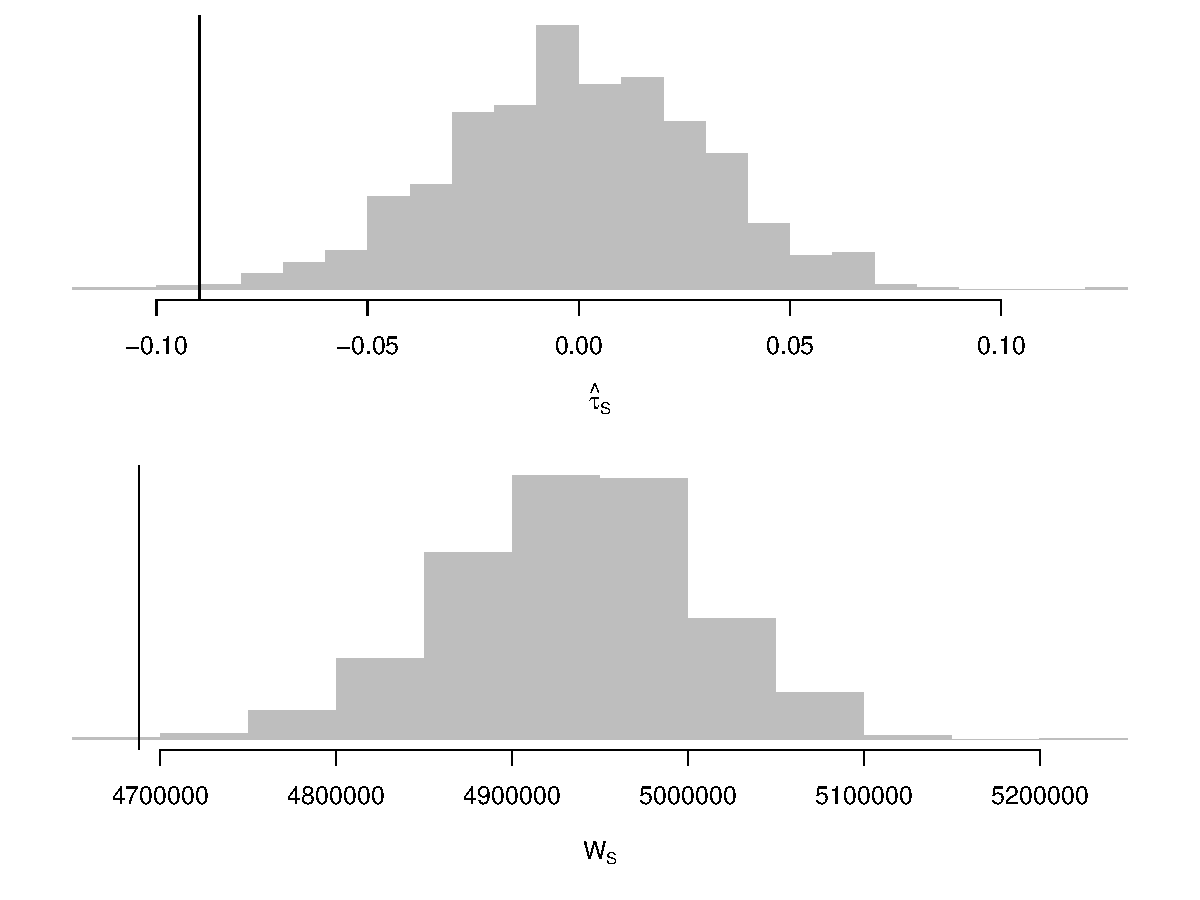
\includegraphics[width = \textwidth]{figures/FRT_SRE_histograms.pdf}
\caption{宾州奖金实验中$\hat{\tau}_\textsc{S}$与$W_\textsc{S}$的随机化分布，使用$10^4$次蒙特卡洛抽样}\label{fig::frt_sre_penn}
\end{figure} 



\section{内曼推断法}
\label{sec::sre-neyman}
\subsection{点估计与区间估计}

分层随机实验本质上由$K$个独立的完全随机实验组成，据此可推广\citet{Neyman:1923}的结论。第$k$层内，均值差$\hat{\tau}_{[k]}$是$\tau_{[k]}$的无偏估计，方差为
$$
\var ( \hat{\tau}_{[k]}) =  \frac{S_{[k]}^2(1)}{ n_{[k]1} } +  \frac{S_{[k]}^2(0)}{ n_{[k]0} }
- \frac{  S_{[k]}^2(\tau) }{ n_{[k]} },
$$
其中$ S_{[k]}^2(1), S_{[k]}^2(0)$与$S_{[k]}^2(\tau)$分别为层内潜在结果和个体因果效应的方差。因此，分层估计量$\hat{\tau}_\textsc{S} = \sum_{k=1}^K  \pi_{[k]} \hat{\tau}_{[k]}$是$\tau =\sum_{k=1}^K  \pi_{[k]}  \tau_{[k]} $的无偏估计，方差为
$$
\var( \hat{\tau}_\textsc{S}   ) = \sum_{k=1}^K  \pi_{[k]}^2   \var ( \hat{\tau}_{[k]}).
$$
若$n_{[k]1} \geq 2$且$n_{[k]0} \geq 2$，可计算第$k$层内结果的样本方差$\hat{S}_{[k]}^2(1)$与$\hat{S}_{[k]}^2(0)$，并构造保守方差估计量
$$
\hat{V}_\textsc{S}  = \sum_{k=1}^K  \pi_{[k]}^2 \left(  \frac{\hat{S}_{[k]}^2(1)}{ n_{[k]1} } +  \frac{ \hat{S}_{[k]}^2(0)}{ n_{[k]0} } \right), 
$$
其中$\hat{S}_{[k]}^2(1)$和$\hat{S}_{[k]}^2(0)$分别为各层处理组与对照组结果的样本方差。对$\hat{\tau}_\textsc{S} $作正态近似，可构造$\tau$的 Wald 型$1-\alpha$置信区间：
$$
\hat{\tau}_\textsc{S} \pm z_{1-\alpha/2} \sqrt{  \hat{V}_\textsc{S}  } . 
$$
从检验角度，在$\HN: \tau=0$下，可将$t_\textsc{S} =   \hat{\tau}_\textsc{S} / \sqrt{  \hat{V}_\textsc{S}  }$与标准正态分位点比较，得到渐近$p$值。统计量$t_\textsc{S} $也出现在例\ref{eg::student-stratifiedestimator}的 FRT 中。后文第\ref{chapter::unification-fisher-neyman}章将证明，以$t_\textsc{S} $进行 FRT，在$\HF$下给出有限样本精确$p$值，在$\HN$下给出渐近有效$p$值。 



这里略去$\hat{\tau}_\textsc{S} $中心极限定理的技术细节。\citet{liu2020regression}给出了证明，同时覆盖少数大层与许多小层两种渐近情形。后文第\ref{sec::sre-neyman-example}节通过数值例子说明这一理论问题。 


\subsection{数值示例}
\label{sec::sre-neyman-example}

下面的函数计算分层随机实验的 Neyman 点估计和方差估计：
\begin{lstlisting}
Neyman_SRE = function(z, y, x)
{
       xlevels = unique(x)
       K       = length(xlevels)
       PiK     = rep(0, K)
       TauK    = rep(0, K)
       varK    = rep(0, K)
       for(k in 1:K)
       {
             xk         = xlevels[k]
             zk         = z[x == xk]
             yk         = y[x == xk]
             PiK[k]     = length(zk)/length(z)
             TauK[k]    = mean(yk[zk==1]) - mean(yk[zk==0])
             varK[k]    = var(yk[zk==1])/sum(zk) + 
                               var(yk[zk==0])/sum(1 - zk)
       }
       
       return(c(sum(PiK*TauK), sum(PiK^2*varK)))
}
\end{lstlisting} 


第一个模拟设定取$K=5$，每层$80$个单位。\ri{TauHat}和\ri{VarHat}分别保存$10^4$次模拟的点估计与方差估计。 
\begin{lstlisting}
> K  = 5
> n  = 80
> n1 = 50
> n0 = 30
> x  = rep(1:K, each = n)
> y0 = rexp(n*K, rate = x)
> y1 = y0 + 1
> zb = c(rep(1, n1), rep(0, n0))
> MC = 10^4
> TauHat = rep(0, MC)
> VarHat = rep(0, MC)
> for(mc in 1:MC)
+ {
+   z  = replicate(K, sample(zb))
+   z  = as.vector(z)
+   y  = z*y1 + (1-z)*y0
+   est = Neyman_SRE(z, y, x) 
+   TauHat[mc] = est[1]
+   VarHat[mc] = est[2]
+ }
> var(TauHat)
[1] 0.002248925
> mean(VarHat)
[1] 0.002266396
\end{lstlisting} 
图\ref{fig::2CLTs}上图给出点估计量的直方图，它围绕真实参数对称，呈钟形。由于个体因果效应恒定，方差估计量的平均值几乎等于点估计量的真实方差。 



第二个模拟设定取$K=50$，每层$8$个单位。 
\begin{lstlisting}
> K  = 50
> n  = 8
> n1 = 5
> n0 = 3
> x  = rep(1:K, each = n)
> y0 = rexp(n*K, rate = log(x + 1))
> y1 = y0 + 1
> zb = c(rep(1, n1), rep(0, n0))
> MC = 10^4
> TauHat = rep(0, MC)
> VarHat = rep(0, MC)
> for(mc in 1:MC)
+ {
+   z  = replicate(K, sample(zb))
+   z  = as.vector(z)
+   y  = z*y1 + (1-z)*y0
+   est = Neyman_SRE(z, y, x) 
+   TauHat[mc] = est[1]
+   VarHat[mc] = est[2]
+ }
> 
> hist(TauHat, xlab = expression(hat(tau)[S]),
+      ylab = "", main = "many small strata", 
+      border = FALSE, col = "grey",
+      breaks = 30, yaxt = 'n',
+      xlim = c(0.8, 1.2))
> abline(v = 1)
> 
> var(TauHat)
[1] 0.001443111
> mean(VarHat)
[1] 0.001473616
\end{lstlisting} 
图\ref{fig::2CLTs}下图给出点估计量的直方图，它同样围绕真实参数对称，呈钟形。由于个体因果效应恒定，方差估计的平均值再次几乎等于点估计量的真实方差。 

\begin{figure}
\centering
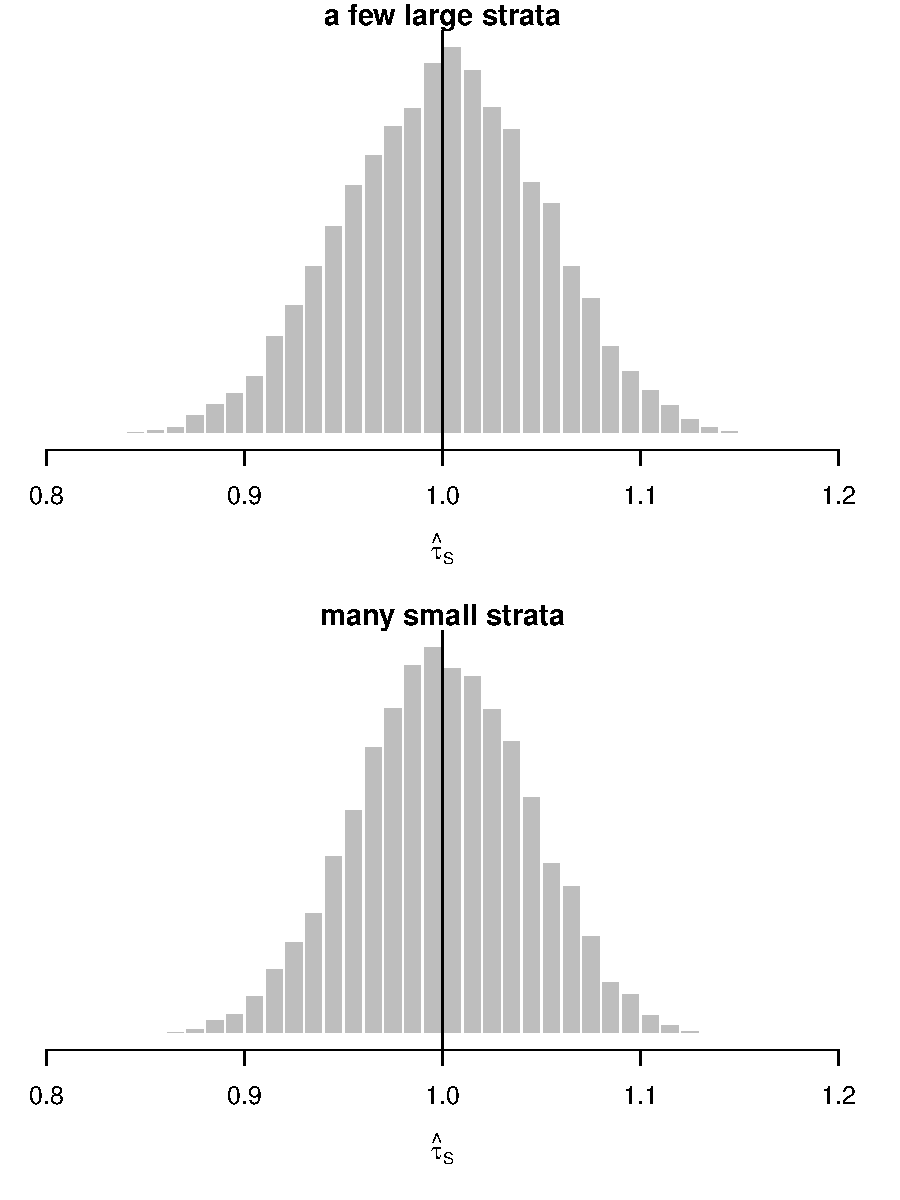
\includegraphics[width = \textwidth]{figures/SRE_CLT_2Regimes.pdf}
\caption{两种分层规模的渐近正态性表现}\label{fig::2CLTs}
\end{figure} 




最后以宾州奖金实验说明分层随机实验的 Neyman 推断。对数据使用\ri{Neyman_SRE}函数，得到：
\begin{lstlisting}
> penndata = read.table("Penn46_ascii.txt")
> z = penndata$treatment
> y = log(penndata$duration)
> block = penndata$quarter
> est = Neyman_SRE(z, y, block)
> est[1]
[1] -0.08990646
> sqrt(est[2])
[1] 0.03079775
\end{lstlisting} 
因此，该职业培训项目显著缩短了就业前等待时长的对数。 


\subsection{比较分层随机实验与完全随机实验}

分层随机实验相比完全随机实验有什么好处？前面从协变量平衡出发引入分层设计，下面说明更好的平衡还能提高平均因果效应的估计精度。为公平比较，假定对所有$k$都有$e_{[k]} = e$，此时均值差等于分层估计量：
\begin{equation}
\label{eq::dim=stratified}
\hat{\tau} = \hat{\tau}_\textsc{S}.
\end{equation}
\eqref{eq::dim=stratified}的证明留作习题\ref{hw::sre-additional-neyman}。 




下面比较抽样方差。经典方差分析将总方差分解为层内方差与层间方差，得到
\begin{eqnarray*}
S^2(1) &=&  (n-1)^{-1} \sumn \{  Y_i(1) - \bar{Y}(1) \}^2 \\
&=& (n-1)^{-1} \sum_{k=1}^K \sum_{X_i   = k} \{ Y_i(1) - \bar{Y}_{[k]}(1)  + \bar{Y}_{[k]}(1)  -   \bar{Y}(1)  \}^2 \\
&=& (n-1)^{-1} \sum_{k=1}^K \sum_{X_i   = k} \left[  \{ Y_i(1) - \bar{Y}_{[k]}(1) \}^2 +  \{ \bar{Y}_{[k]}(1)  -   \bar{Y}(1)  \}^2 \right] \\
&=& \sum_{k=1}^K \left[   \frac{n_{[k]} - 1}{n-1}   S_{[k]}^2(1)  +  \frac{ n_{[k]}}{ n-1} \{ \bar{Y}_{[k]}(1) - \bar{Y}(1) \}^2  \right],
\end{eqnarray*}
类似地，
\begin{eqnarray*}
S^2(0) &=& \sum_{k=1}^K \left[   \frac{n_{[k]} - 1}{n-1}   S_{[k]}^2(0)  +  \frac{ n_{[k]}}{ n-1} \{ \bar{Y}_{[k]}(0) - \bar{Y}(0) \}^2  \right],\\
S^2(\tau) &=& \sum_{k=1}^K \left[   \frac{n_{[k]} - 1}{n-1}   S_{[k]}^2(\tau)  +  \frac{ n_{[k]}}{ n-1} \{ \tau_{[k]} - \tau \}^2  \right] .
\end{eqnarray*}
完全随机实验下均值差估计量的方差可分解为
\begin{eqnarray*}
&&\var_{\text{CRE}}(  \hat{\tau} )  \\
&=& \frac{S^2(1)}{ n_{1} } +  \frac{S^2(0)}{ n_{0} }
- \frac{  S^2(\tau) }{ n }  \\ 
&=& \sum_{k=1}^K  \left[   \frac{ n_{[k]} - 1}{(n-1)n_1}  S_{[k]}^2(1) + \frac{ n_{[k]} - 1}{ (n-1)n_0}  S_{[k]}^2(0) -  \frac{ n_{[k]} - 1}{(n-1)n}    S_{[k]}^2(\tau) \right] \\
&&  + \sum_{k=1}^K  \left[    \frac{ n_{[k]} - 1}{ (n-1)n_1}  \{ \bar{Y}_{[k]}(1) - \bar{Y}(1) \}^2 +  \frac{ n_{[k]} - 1}{ (n-1)n_0}  \{ \bar{Y}_{[k]}(0) - \bar{Y}(0) \}^2   \right. \\
&& \left.  - \frac{ n_{[k]} - 1  }{ (n-1)n} \{ \tau_{[k]} - \tau \}^2  \right] .
 \end{eqnarray*}
各$n_{[k]}$较大时，近似为
\begin{eqnarray*}
 &&\var_{\text{CRE}}(  \hat{\tau} )  \\
&\approx & 
\sum_{k=1}^K  \left[   \frac{ \pi_{[k]}}{n_1}  S_{[k]}^2(1) + \frac{ \pi_{[k]}}{n_0}  S_{[k]}^2(0) -  \frac{ \pi_{[k]}}{n}    S_{[k]}^2(\tau) \right] \\
&&  + \sum_{k=1}^K  \left[    \frac{ \pi_{[k]}}{n_1}  \{ \bar{Y}_{[k]}(1) - \bar{Y}(1) \}^2 +  \frac{ \pi_{[k]}}{n_0}  \{ \bar{Y}_{[k]}(0) - \bar{Y}(0) \}^2  
 - \frac{ \pi_{[k]}  }{n} \{ \tau_{[k]} - \tau \}^2  \right] .
\end{eqnarray*}
恒定倾向得分假设保证
$$ 
\pi_{[k]} / n_{[k]1}  = 1/(ne), \quad   \pi_{[k]} / n_{[k]0} = 1/\{n(1-e) \},\quad \pi_{[k]} / n_{[k]} = 1/n,
$$
从而可将分层随机实验中$\hat{\tau}_\textsc{S}$的方差改写为
\begin{eqnarray*}
\var_\textsc{SRE}(\hat{\tau}_\textsc{S}) &= & \sum_{k=1}^K  \pi_{[k]}^2 \left[ \frac{S_{[k]}^2(1)}{ n_{[k]1} } +  \frac{S_{[k]}^2(0)}{ n_{[k]0} }
- \frac{  S_{[k]}^2(\tau) }{ n_{[k]} } \right]\\
&=&\sum_{k=1}^K  \left[   \frac{ \pi_{[k]}}{n_1}  S_{[k]}^2(1) + \frac{ \pi_{[k]}}{n_0}  S_{[k]}^2(0) -  \frac{ \pi_{[k]}}{n}    S_{[k]}^2(\tau) \right] .
\end{eqnarray*}
各$n_{[k]}$较大时，$\var_{\text{CRE}}(  \hat{\tau} )$与$\var_\textsc{SRE}(\hat{\tau}_\textsc{S})$之差近似为
$$
\sum_{k=1}^K  \left[    \frac{ \pi_{[k]}}{n_1}  \{ \bar{Y}_{[k]}(1) - \bar{Y}(1) \}^2 +  \frac{ \pi_{[k]}}{n_0}  \{ \bar{Y}_{[k]}(0) - \bar{Y}(0) \}^2  
 - \frac{  \pi_{[k]}  }{n}  ( \tau_{[k]} - \tau  ) ^2  \right] 
 $$
这一差值非负，因为它等于（见习题\ref{hw::compare-CRE-SRE}）
\begin{eqnarray}
\label{eq::difference}
\sum_{k=1}^K\frac{ \pi_{[k]}}{n} 
 \left\{
\sqrt{ \frac{n_0}{n_1} } \{ \bar{Y}_{[k]}(1) - \bar{Y}(1) \} +  \sqrt{ \frac{n_1}{n_0} } \{ \bar{Y}_{[k]}(0) - \bar{Y}(0) \}
 \right\}^2 \geq 0,
\end{eqnarray}
\eqref{eq::difference}仅在对所有$k=1,\ldots, K$均有
$$
\sqrt{ \frac{n_0}{n_1} } \{ \bar{Y}_{[k]}(1) - \bar{Y}(1) \} +  \sqrt{ \frac{n_1}{n_0} } \{ \bar{Y}_{[k]}(0) - \bar{Y}(0) \}
= 0 
$$
的极端情况下为零。若协变量能预测潜在结果，上述各量通常不全为零，因而分层随机实验比完全随机实验更有效率。只有协变量完全没有预测能力的极端情形，大样本效率增益才为零；此时在有限样本中，分层甚至可能降低效率。这呼应了本章开头 George Box 的名言。 

 


最后补充几点。第一，上述比较针对抽样方差，也可比较两种设计下的估计方差，结论类似。第二，增加$K$能提高效率，但论证依赖各层足够大的假设，因此实践中存在权衡。不能任意增大$K$；最极端的情形是$n_{[k]1} = n_{[k]0} = 1$，即第\ref{chapter::mpe}章将介绍的配对实验。 

 




\section{完全随机实验中的后分层}\label{sec::poststra-cre}

在具有离散协变量$X$的完全随机实验中，第$k$层的处理与对照单位数随机；在分层随机实验中，这些数固定。但若给定$\bm{n} = \{  n_{[k]1} , n_{[k]0} \}_{k=1}^K$作条件推断，完全随机实验就变为分层随机实验。从数学上说，若$\bm{n}$的各分量均不为零，则
\begin{equation}\label{eq::condition-to-SRE}
\pr_\textsc{CRE}(\bm{Z} = \bm{z} \mid\bm{n} )
= \frac{ \pr_\textsc{CRE}( \bm{Z} = \bm{z},  \bm{n})   }{ \pr_\textsc{CRE}(   \bm{n})   }
=  \frac{1}{  \prod_{k=1}^K  \binom{  n_{[k]} }{  n_{[k]1} } }  ,
\end{equation}
即完全随机实验中给定$\bm{n}$后$\bm{Z}$的条件分布，与分层随机实验中$\bm{Z}$的分布相同。\eqref{eq::condition-to-SRE}的证明留作习题\ref{hw::CRE-SRE}。因此，给定$\bm{n}$后，可按分层随机实验的方法分析带离散协变量$X$的完全随机实验。具体而言，FRT 变为{\it 条件 FRT}，Neyman 分析变为{\it 后分层}：
$$
\hat{\tau}_\textsc{PS} = \sum_{k=1}^K \pi_{[k]} \hat{\tau}_{[k]},
$$
其形式与$\hat{\tau}_\textsc{S}$相同。给定$\bm{n}$时$\hat{\tau}_\textsc{PS} $的方差，等于分层随机实验下$\hat{\tau}_\textsc{S}$的方差。  


\citet{hennessy2016conditional}通过模拟表明，条件 FRT 的功效往往高于无条件 FRT。\citet{miratrix:2013}从理论上证明，后分层在许多情形下比$\hat{\tau}$更有效率。二者都要求$X$能预测结果。但模拟只覆盖有限的数据生成过程，理论也要求各层足够大。条件 FRT 或后分层不能划分得过细：$K$越大，某些$n_{[k]1} $或$ n_{[k]0}$为零的可能性越高。$n_{[k]1} $或$ n_{[k]0}$很小甚至为零时，FRT 的可行随机分配数大幅减少，功效可能显著降低。Neyman 推断的问题更明显，因为此时甚至无法定义$\hat{\tau}_\textsc{PS}$及其方差估计量。 


分层在设计阶段使用$X$，后分层在分析阶段使用$X$，二者是利用$X$的对偶方法。当各层较大时，两者的差异渐近较小\citep{miratrix:2013}。

\subsection{\citet{meinert1970study}的例子}\label{sec::ps-merinert}

使用\citet{meinert1970study}报告的完全随机实验数据，\citet{rothman2008modern}也曾使用这组数据。处理为甲苯磺丁脲，对照为安慰剂。 
\begin{center} 
\begin{tabular}{ccc}
\multicolumn{3}{c}{ 年龄 $< 55$} \\
\hline 
 & 存活 & 死亡 \\
$Z=1$ &    98 & 8 \\
$Z=0$  & 115 & 5 \\
\hline 
\end{tabular}
%&
\begin{tabular}{ccc}
\multicolumn{3}{c}{ 年龄 $\geq  55$} \\
\hline 
 & 存活 & 死亡 \\
$Z=1$ &    76 & 22 \\
$Z=0$  &  69 & 16 \\
\hline 
\end{tabular}
%&
\begin{tabular}{ccc}
\multicolumn{3}{c}{合计 } \\
\hline 
 & 存活 & 死亡 \\
$Z=1$ &    174 & 30 \\
$Z=0$  & 184 & 21 \\
\hline 
\end{tabular}
\end{center}
 

下表分别给出两层的估计量、后分层估计量、忽略二元协变量的粗估计量，以及各自的标准误。  
\begin{center}
\begin{tabular}{crrrr}
\hline 
    &第 1 层& 第 2 层 &后分层 &  未调整 \\
估计值 &    $-0.034$ &   $-0.036$ &  $-0.035$ & $-0.045$ \\
标准误   &   $0.031$    & $0.060$   & $0.032$   & $0.033$\\
\hline 
\end{tabular}
\end{center} 


粗估计与后分层估计没有给出根本不同的结论。但粗估计大于两个层内估计，而后分层估计位于二者之间。 


\subsection{\citet{chong2016iron}的例子}\label{sec::ps-chong}


\citet{chong2016iron}在 2009 学年，对秘鲁 Cajamarca 地区一所农村中学的 219 名学生实施了分层随机实验。研究者先向村诊所提供铁补充剂，并培训工作人员，让亲自前来领取的青少年免费获得铁片。随后随机分配学生观看三类视频：第一类由知名足球运动员鼓励服用铁剂以提高精力（“足球”组）；第二类由医生鼓励服用铁剂以改善总体健康（“医生”组）；第三类完全不提铁剂（“对照”组）。实验按年级（1—5）分层，各层的处理与对照人数如下：

\begin{lstlisting}
> library("foreign")
> dat_chong = read.dta("chong.dta")
> table(dat_chong$treatment, dat_chong$class_level)
               
                 1  2  3  4  5
  Soccer Player 16 19 15 10 10
  Physician     17 20 15 11 10
  Placebo       15 19 16 12 10
\end{lstlisting}

关注的一个结果是 2009 年第三、第四季度的平均成绩，重要的背景协变量是基线贫血状况。本章只使用原数据的一个子集。 

\begin{lstlisting}
> use.vars = c("treatment", 
+              "gradesq34", 
+              "class_level", 
+              "anemic_base_re")
> dat_physician = subset(dat_chong,
+                        treatment != "Soccer Player",
+                        select = use.vars)
> dat_physician$z = (dat_physician$treatment=="Physician")
> dat_physician$y = dat_physician$gradesq34
> table(dat_physician$z, 
+       dat_physician$class_level)
       
         1  2  3  4  5
  FALSE 15 19 16 12 10
  TRUE  17 20 15 11 10
> table(dat_physician$z, 
+       dat_physician$class_level,
+       dat_physician$anemic_base_re)
, ,  = No

       
         1  2  3  4  5
  FALSE  6 14 12  7  4
  TRUE   8 12  9  5  6

, ,  = Yes

       
         1  2  3  4  5
  FALSE  9  5  4  5  6
  TRUE   9  8  6  6  4
\end{lstlisting}

 
可使用前面定义的\ri{Neyman_SRE}函数，计算分层估计量及其估计方差。 
\begin{lstlisting}
tauS = with(dat_physician,
            Neyman_SRE(z, gradesq34, class_level))
\end{lstlisting}

另一个重要协变量是基线贫血指标，它对预测结果十分重要。进一步以基线贫血状态分层，得到$5\times 2 =10$个层，各层处理与对照人数如上。仍可使用此前的\ri{Neyman_SRE}函数，计算后分层估计量及其方差估计。 
 \begin{lstlisting}
> tauSPS = with(dat_physician, {
+   sps = interaction(class_level, anemic_base_re)
+   Neyman_SRE(z, gradesq34, sps)
+ })
\end{lstlisting}

下表比较两个估计量，后分层估计得到的$p$值明显更小。 
\begin{center}
\begin{tabular}{crrrr}
                          & 估计值 &   标准误 &t 统计量& p 值 \\
分层                & 0.406 &0.202 & 2.005  & 0.045 \\
分层与后分层 & 0.463 &0.190 & 2.434 &  0.015
\end{tabular}
\end{center} 

这个例子表明，后分层不仅适用于完全随机实验，也适用于具有额外离散协变量的分层随机实验。 


\section{实践注意事项}


应如何选择$X$来构造分层随机实验？理论上，$X$应能预测潜在结果。有时实验者根据先导研究等已充分了解哪些协变量有预测能力，选择$X$就很直接。其他情况下，背景知识可能不足，实验者就按实施便利选择$X$，例如用$X$表示研究地区或学生届别。 


层数$K$的选择是相关问题。理论上，只要各层足够大，分层越细，估计效率越高；但$K$过大反而可能降低效率。模拟中，增加$K$的边际收益会递减。经验上，$K = 5$往往已经足以带来效率增益（这个神奇数字$5$将在第\ref{chapter::pscore-key}章再次出现）。有些实验者偏好分层随机实验的最极端版本$K=n/2$，即后文第\ref{chapter::mpe}章介绍的配对实验。  


若实验有多维连续协变量，还能使用分层设计吗？若有先导研究，可根据这些协变量建立潜在结果$Y(0)$的预测模型，再以预测值$\hat{Y}(0)$的离散化版本作为$X$。若没有这样的先导研究，或不愿作人为离散化，则可使用更一般的再随机化策略，这是第\ref{chapter:rerandomization-regression}章的主题。 

 
 
 \section{作业习题}
 
 
  \paragraph{常规实验中的协变量平衡}\label{hw::balance-discrete-CRE}
  
 在完全随机实验下，证明 \eqref{eq::balance-discrete-CRE}。 
 
 \paragraph{恒定因果效应的影响}
\label{hw::sre-additional-neyman}

证明 \eqref{eq::dim=stratified}。 


\paragraph{个体因果效应恒定的推论}

假定对所有$i=1,\ldots, n$都有恒定个体因果效应$\tau_i = \tau$。考虑以下$\tau$的加权估计量族：
$$
\hat{\tau}_w = \sum_{k=1}^K  w_{[k]}  \hat{\tau}_{[k]} ,
$$
其中对所有$k$，权重$w_{[k]}  $均非负。

求权重$w_{[k]}$满足什么条件时，$\hat{\tau}_w $是$\tau$的无偏估计。在所有无偏估计量中，找出使$\hat{\tau}_w$方差最小的权重。 


\paragraph{两种实验设计的差异}\label{hw::compare-CRE-SRE}

证明 \eqref{eq::difference}。



\paragraph{条件分布转化}\label{hw::CRE-SRE}


证明 \eqref{eq::condition-to-SRE}。


 
 \paragraph{第\ref{sec::frt-pennbonus}节的其他 FRT}\label{hw::FRT-SRE-more}
 
 使用其他检验统计量的 FRT，推广第\ref{sec::frt-pennbonus}节的分析。


 
 \paragraph{\citet{imbens2015causal} 实例分析}
重现 STAR 实验的分层后推断过程。


\citet{imbens2015causal}讨论了 1985—1986 年在田纳西州开展的学生／教师比例实验中的分层随机实验。幼儿园数据如下：
 \begin{lstlisting}
treatment = list(c(1,1,0,0), 
                 c(1,1,0,0), 
                 c(1,1,1,0,0), 
                 c(1,1,0,0),
                 c(1,1,0,0),
                 c(1,1,0,0),
                 c(1,1,0,0), 
                 c(1,1,1,1,0,0),
                 c(1,1,0,0),
                 c(1,1,0,0),
                 c(1,1,0,0),
                 c(1,1,1,0,0),
                 c(1,1,0,0),
                 c(1,1,0,0),
                 c(1,1,0,0),
                 c(1,1,0,0))
outcome = list(c(0.165,0.321,-0.197,0.236), 
               c(0.918,-0.202,1.19,0.117),
               c(0.341,0.561,-0.059,-0.496,0.225),
               c(-0.024,-0.450,-1.104,-0.956), 
               c(-0.258,-0.083,-0.126,0.106),
               c(1.151,0.707,0.597,-0.495), 
               c(0.077,0.371,0.685,0.270), 
               c(-0.870,-0.496,-0.444,0.392,-0.934,-0.633), 
               c(-0.568,-1.189,-0.891,-0.856), 
               c(-0.727,-0.580,-0.473,-0.807), 
               c(-0.533,0.458,-0.383,0.313), 
               c(1.001,0.102,0.484,0.474,0.140), 
               c(0.855,0.509,0.205,0.296), 
               c(0.618,0.978,0.742,0.175), 
               c(-0.545,0.234,-0.434,-0.293), 
               c(-0.240,-0.150,0.355,-0.130))
\end{lstlisting}
各层对应学校，分析单位为教师或班级。小班（每位教师 13—17 名学生）的处理取$1$，常规班（每位教师 22—25 名学生）取$0$。结果为标准化数学平均成绩。


用 FRT 重新分析下面的 STAR 项目数据，分别使用$\hat{\tau}_\textsc{S}$、$W_\textsc{S}$和$\tilde W$，比较$p$值。

注：本书用$Z$表示处理指标，\citet{imbens2015causal}使用$W.$。
 






\paragraph{数据再分析}

\citet[][Table 1]{gould1998multi}报告了一项多中心试验的数据：

\begin{lstlisting}
> multicenter = read.csv("multicenter.csv")
> multicenter
   center n0 mean0  sd0 n1 mean1  sd1 n5 mean5  sd5
1       1  7  0.43 4.58  7 -5.43 5.53  8 -2.63 3.38
2       2 11  0.10 4.21 11 -2.59 3.95 12 -2.21 4.14
3       3  6  2.58 4.80  6 -3.94 4.25  7  1.29 7.39
4       4 10 -2.30 3.86 10 -1.23 5.17 10 -1.40 2.27
5       5 10  2.08 6.46 10 -6.70 7.45 10 -5.13 3.91
6       6  6  1.13 3.24  5  3.40 8.17  5 -1.59 3.19
7       7  5  1.20 7.85  6 -3.67 4.89  5 -1.40 2.61
8       8 12 -1.21 2.66 13  0.18 3.81 12 -4.08 6.32
9       9  8  1.13 5.28  8 -2.19 5.17  9 -1.96 5.84
10     10  9 -0.11 3.62 10 -2.00 5.35 10  0.60 3.53
11     11 15 -4.37 6.12 14 -2.68 5.34 15 -2.14 4.27
12     12  8 -1.06 5.27  9  0.44 4.39  9 -2.03 5.76
13     13 12 -0.08 3.32 12 -4.60 6.16 11 -6.22 5.33
14     14  9  0.00 5.20  9 -0.25 8.23  7 -3.29 5.12
15     15  6  1.83 5.85  7 -1.23 4.33  6 -1.00 2.61
16     16 14 -4.21 7.53 14 -2.10 5.78 12 -5.75 5.63
17     17 13  0.76 3.82 13  0.55 2.53 13 -0.63 5.41
18     18 15 -1.05 4.54 13  2.54 4.16 14 -2.80 2.89
19     19 15  2.07 4.88 15 -1.67 4.95 15 -3.43 4.71
20     20 11 -1.46 5.48 10 -1.99 5.63 10 -6.77 5.19
21     21  5  0.80 4.21  5 -3.35 4.73  5 -0.23 4.14
22     22 11 -2.92 5.42 10 -1.22 5.95 11 -4.45 6.65
23     23  9 -3.37 4.73  9 -1.38 4.17  7  0.57 2.70
24     24 12 -1.92 2.91 12 -0.66 3.55 12 -2.39 2.27
25     25  9 -3.89 4.76  9 -3.22 5.54  8 -1.23 4.91
26     26 15 -3.48 5.98 15 -2.13 3.25 14 -3.71 5.30
27     27 11 -1.91 6.49 12 -1.33 4.40 11 -1.52 4.68
28     28 10 -2.66 3.80 10 -1.29 3.18 10 -4.70 3.43
29     29 13 -0.77 4.73 13 -2.31 3.88 13 -0.47 4.95
\end{lstlisting}


这是以研究中心为层的分层随机实验，用于研究非那雄胺治疗良性前列腺增生的疗效与耐受性。在$29$个中心内，分别将患者随机分为对照、1 mg 非那雄胺和 5 mg 非那雄胺三组。数据给出了结果的汇总统计量；结果为总症状评分相对于基线的变化。总症状评分是九个反映排尿能力受损不同方面的问题得分之和，每题取$0$至$4$分。各列含义如下：

\begin{enumerate}
\item
\texttt{center}：研究中心编号；
\item
\texttt{n0, n1, n5}：三个组的样本量；
\item
\texttt{mean0, mean1, mean5}：三个组的结果均值；
\item
\texttt{sd0, sd1, sd5}：三个组的结果标准差。 
\end{enumerate}

未报告个体结果，因此无法实施 FRT。但 Neyman 推断只需汇总统计量。请分别比较“1 mg 非那雄胺”与“对照”、“5 mg 非那雄胺”与“对照”，报告点估计和方差估计。 


\paragraph{数据再分析}
 
 
重新分析第\ref{sec::example-neyman-formula}节使用的 LaLonde 数据，同时进行 Fisher 推断和 Neyman 推断。 

原实验为完全随机实验，现在假装它采用分层随机设计，分别重新分析：(1) 按种族（黑人、西班牙裔、其他）分层；(2) 按婚姻状况分层；(3) 按是否有高中毕业文凭分层。 

与完全随机实验下的结果比较。 

 


\paragraph{推荐阅读}

\citet{miratrix:2013}为后分层提供了严格理论，并将其与分层比较。主要结论是：尽管有限样本下二者可能不同，渐近差异较小。 



